\documentclass[10pt,a4paper]{article}
\usepackage[utf8]{inputenc}
\usepackage{amsmath}
\usepackage{amsfonts}
\usepackage{amssymb}
\usepackage{graphicx}
\usepackage[left=2cm,right=2cm,top=2cm,bottom=2cm]{geometry}
\author{Joshua Stubbs}
\title{Documentation for "nav-only"}
\begin{document}
\maketitle
\noindent



\section{General}
Nav-only is a modification of the main Pyxis code that enables the user to run the receiver quicker by inputting an existing APT (Amplitude Phase Time) binary file. RNX binaries (used for positioning, and is the main file for analysing the results of a run) or KML files (for Google Earth) can be outputted. \subsection{System Requirements}
The code has been tested on a 64 bit machine running LinuxMint 17.2, and this is recommended for operation. Ubuntu will likely work too. \\ \\
\noindent
Before running anything a few things need to be fixed;
\begin{itemize}
\item Run the following commands in a terminal window to install the required packages:
\begin{itemize}
\item \textbf{sudo apt-get update; sudo apt-get upgrade -y; sudo apt-get dist-upgrade -y}
\item \textbf{sudo apt-get install build-essential doxygen graphviz texlive-latex-extra texlive-latex-base texlive-latex-recommended texlive-fonts-recommended latex-xcolor check}
\end{itemize} 
\item Run the script "remakePath.sh" by navigating to (in a terminal window) stand\_alone\_nav/largeFiles and then running it by typing "./remakePath.sh"
\end{itemize}



\section{Important Files}
\label{sec:files}
The code should be setup to run everything, without having to change any file paths. However, if you do want to change how the code is run, the following files are important: \\ \\
\noindent
The first file of importance is "conf.h" (located in /src/conf). Make sure that \textbf{NAVDEBUG} is set to 1, and then that the appropriate outputs (such as RNX) are enabled. Note that LOGAPT is set to 0 regardless of selection. \\ \\
\noindent
The second file of importance is "conf\_swc.h" (located in /src/conf). This is where you will give the input/output file paths. Even though \textbf{APTOUT} was disabled in "conf.h" the file path needs to be defined here too, as it will actually specify the \textit{input} path to the existing APT file. \textbf{KMLOUT} and \textbf{RNXOUT} will specify the output paths of the KML file and RNX binaries. Note that in the code the input file name of \textbf{APTOUT} has to use the \_\%d\_\%d naming convention, or the code will bug (described in more detail in section \ref{sec:prob0} of this document). The actual file has to use the \_0\_0 naming, though.  \\ \\ 
\noindent
Included in the folder is also an APT binary needed to run the code.

\section{Building/Running}
The default setup of the code will read the APT file located in "stand\_alone\_nav/input" and output a RNX binary to "stand\_alone\_nav/output". \\ \\
\noindent
Below the two main methods for building and running the code are described.
\subsection{Terminal}
Building and running the code through the terminal is simple, but offers little assistance in terms of debugging. Editing of files can be done through a text editor of your choice. The necessary steps are:
\begin{enumerate}
\item Open a terminal window
\item Navigate to stand\_alone\_nav/code/build/ directory using the "cd" command
\item run the command "make clean;make" to build the code (needs to be done each time something is changed in any file)
\item run the nav-only code with the command: "../bin/nav/navexe"
\item messages can be seen in the terminal window, and will give a prompt when done. See figure \ref{fig:terminal_success} for what successful operation looks like.
\end{enumerate}


\begin{figure}[h!]
\centering
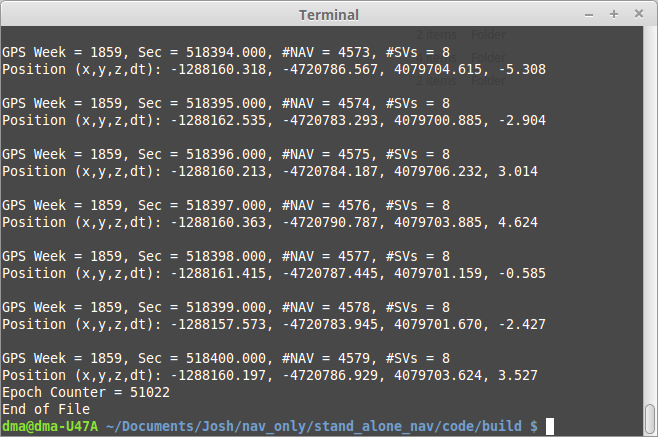
\includegraphics[scale=0.6]{terminal_success.png}
\caption{Successful execution as seen when run in the terminal}
\label{fig:terminal_success}
\end{figure}


\subsection{Eclipse}
\begin{enumerate}
\item Open Eclipse
\item Create a new workspace. This will create a folder of your project name that will be your working directory
\item Click file $\rightarrow$ new $\rightarrow$ project and create a new "C makefile project with existing code".
\item Browse to the "code" folder, and make sure that "C" is selected. Select to use "Linux GCC" as toolchain. Give your project an appropriate name too
\item Click the "Workbench" arrow in the top right corner of the window to open the workspace
\item Click "Open perspective" in the top right corner and select "C/C++"
\item You can now browse your project using the left pane, and edit files as wanted. Set up file paths as described in section \ref{sec:files} of this document
\item Right click your project name in the project explorer and select properties $\rightarrow$ C/C++ Build
\item Under "Build Location" click workspace and select the "build" folder in your code folder. Click "Apply" and "OK" to return to the workspace
\item clean project by selecting the menu option: Project $\rightarrow$ clean $\rightarrow$ clean all
\item click the hammer to build the project
\item select "always run in background" and then click "run in background". Select the "Console" view at the bottom to see what's going on
\item set up how to run the code by going to the "Run" menu and then selecting "Run Configurations"
\item select "C/C++ Application", then click "New launch configuration"
\item (you might have to select your project folder under "Project" before proceeding to the next step)
\item click Browse, and then navigate to the location of "project\_name"/bin/nav/ and select "navexe" (where "project\_name" is the name of your project)
\item click "Apply" and then run to run your code
\item you can now run nav-only by pressing the green play button at top of screen
\item save, clean, build and run the code whenever a file is changed
\end{enumerate}






\section{Post Processing}
To analyse the results of running the above mentioned code some post processing tools are provided in the "stand\_alone\_nav/postProcessing" folder. Their function and operation is described in this section. \\ \\
\noindent
MATLAB is required to run all of the post processing tools. Both scripts have options to change file paths and file names for the input file. As the scripts are currently set up, however, they should work straight away with the generated RNX file.
\subsection{Analyse RNX binary}
The folder "RNX\_Analyser" contains the necessary script to analyse the RNX binary file without converting it. \\ \\
\noindent
Running "AnalysisLSSScript.m" should show a variety of plots and save them in "stand\_alone\_nav/output/RNX\_Analysis"
\subsection{Convert RNX binary to Rinex}
The folder "RNX2Rinex" contains the necessary script to convert your newly created RNX binary to a RINEX file. RINEX is a common file type to use for GPS applications.\\ \\
\noindent
Running "lssBin2RunexScript.m" should create a RINEX file in the "stand\_alone\_nav/output/RINEX\_conversion" folder.







\section{Known Errors}
\subsection{Problem when running "nav-only" with anything else than 0\_0 file}
This issue is a three-part problem; \\ \\
First, only one APT file can be run at the time. When the end of a file is reached, the next one will not be automatically read in as when running the code for the full receiver. \\ \\
Secondly, only the 0\_0 APT file can be read. If any other APT file is input, an error will occur when the ephemeris is updated (see figure \ref{fig:error} below). \\ \\
Thirdly, in order to even read the 0\_0 APT file the input file path has to use the \_\%d\_\%d convention. I.e, your input file is called "aptBinaries\_0\_0.bin",but you have to give the input file name as aptBinaries\_\%d\_\%d.bin.\\ \\

\begin{figure}[h!]
\centering
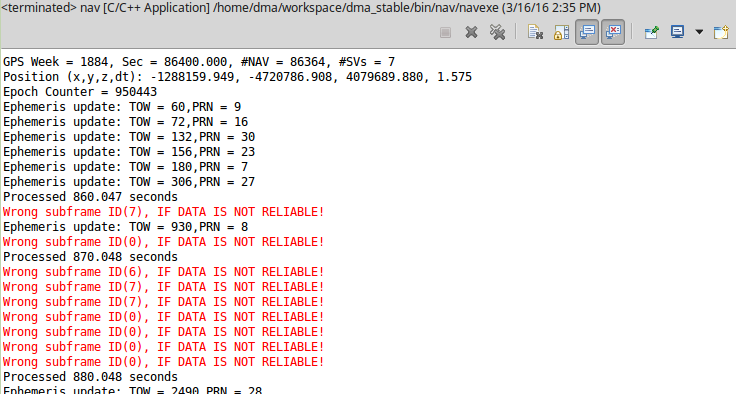
\includegraphics[scale=0.6]{error}
\caption{Error at ephemeris update when not using \_\%d\_\%d system}
\label{fig:error}
\end{figure}
\label{sec:prob0}


\subsection{Eclipse Errors}
Eclipse will sometimes complain about errors on line 0 of the code, but these do not seem to impair operation of the code. \\ \\
\noindent
There is also the possibility of errors occurring when a file is opened and edited in eclipse that contains true or false statements. The code can still be built and run however.

\end{document}